This section describes the rationale behind the thesis and gives a brief introduction to energy disaggregation and its challenges and future prospects. Later, we present the increase in research interest in the field of Non-intrusive load-monitoring (NILM) and lastly present the thesis outline in section \ref{sec:outline}.

Energy issues present one of the largest challenges facing our society. The world currently consumes an average of 16 terawatts of power, 86\% of which comes from fossil fuels; without any effort to curb energy consumption or use of different sources of energy, most climate models predict that the earth’s temperature will increase by at least 3 degrees Celcius in the next 90 years \cite{DDSC}, a change that could cause ecological disasters on a global scale. While there are ofcourse, numerous facets to the energy problem, there is a growing consensus that many energy and sustainability problems are fundamentally a data analysis problem, areas where machine learning can play a significant role.

Perhaps to no surprise, private households have been observed to have some of the largest capacities for improvement when it comes to efficient energy usage. Private households have been observed to have largest capacities for improvement \cite{commision}. However, numerous studies have shown that receiving information about one's energy consumption can automatically induce energy-conserving behaviors \cite{DDSC}, and these studies also clearly indicate that receiving appliance specific information leads to much larger gains than whole-home data alone (\hspace{1sp}\cite{reduce} estimates that appliance-level data could reduce consumption by an average of 12\% in the residential sector). In the United States, electricity constitutes 38\% of all energy used, and residential and commercial buildings together use 75\% of this electricity \cite{DDSC}; thus, this 12\% figure accounts for a sizable amount of energy that could potentially be saved.

Energy Disaggregation, also called Non-Intrusive Load Monitoring (NILM) \cite{hart}, involves taking an aggregated energy signal, for example the total power consumption of a house as read by an electricity meter, and separating it into the different electrical appliances being used. While field surveys and direct measurements of individual appliances have been and still are the most straight forward methods to acquire accurate energy usage data, the need for a multitude of sensors and time consuming installations have made energy disaggregation methods financially unapproachable \cite{jon}. 

Instead, some look specifically at the task of energy disaggregation, via data analytics task relating to energy efficiency. However, the widely-available sensors that provide electricity consumption information, namely the so-called “Smart Meters” that are already becoming ubiquitous, collect energy information only at the whole-home level and at a very low resolution (typically every hour or 15 minutes). Thus, energy disaggregation methods that can take this whole-home data and use it to predict individual appliance usage present an algorithmic challenge, where advances can have a significant impact on large-scale energy efficiency issues. The following figure shows the underlying structure that can happen during an hour of different resolutions.

%\hspace*{-2cm}
\begin{figure}[H]
%	\centering
\hspace*{-0.5cm}
	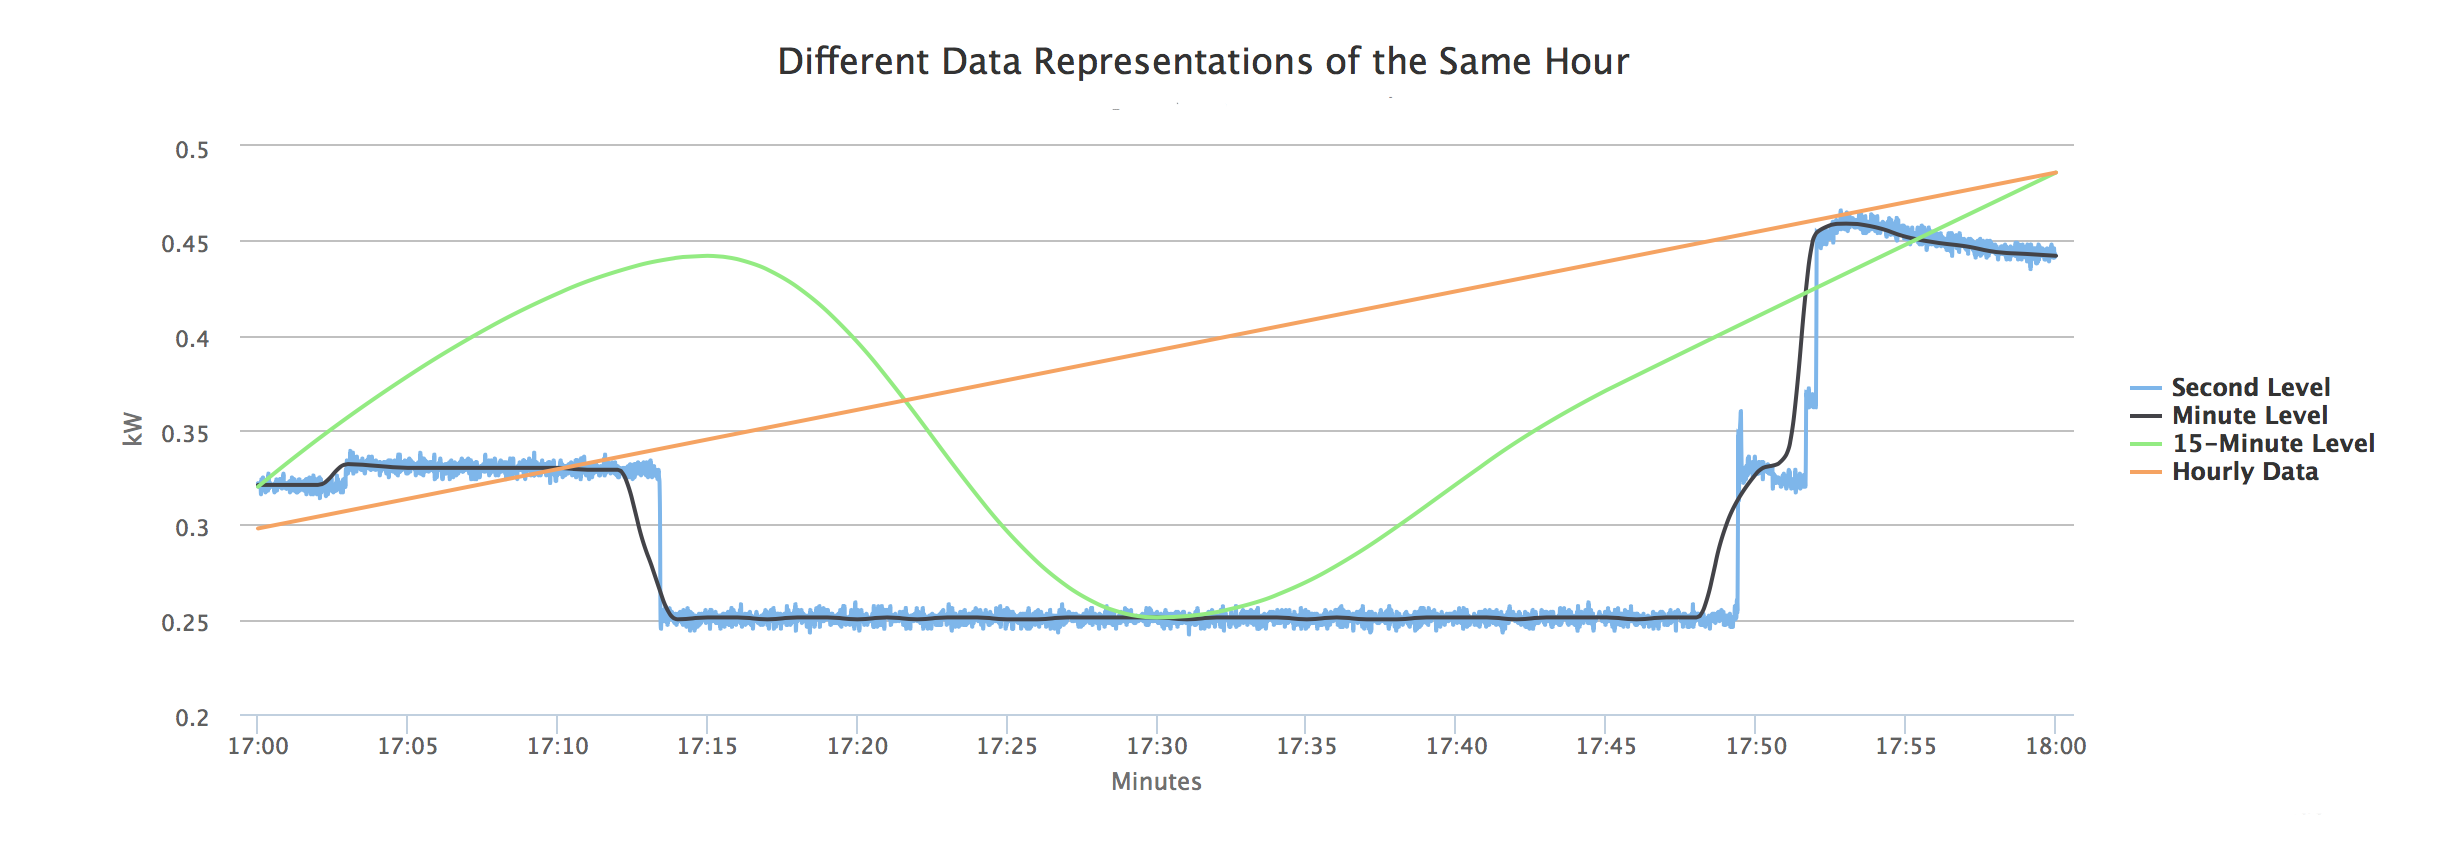
\includegraphics[scale=0.37]{./figures/hourlyexamplefixed.png}
	\caption{A figure to display the difference between low (that of hourly readings) to high resolution data. \protect\footnotemark}
	\label{fig:hourex}
\end{figure}
\footnotetext{Pecan Street Inc, 'Dataport', https://dataport.pecanstreet.org/, (accessed 10 June 2015)}

Energy disaggregation methods do have a long history in the engineering community, including some which have applied machine learning techniques — early algorithms \cite{hart} typically looked for “edges” in power signal to indicate whether a known device was turned on or off; later work focused on computing harmonics of steady-state power or current draw to determine more complex device signatures \cite{load}; recently, researchers have analyzed the transient noise of an electrical circuit that occurs when a device changes state \cite{patel}. However, these and most other studies we are aware of, were either conducted in artificial laboratory environments, contained a relatively small number of devices, trained and tested on the same set of devices in a house, and/or used custom hardware for very high frequency electrical monitoring with an algorithmic focus on “event detection” (detecting when different appliances were turned on and off) \cite{DDSC}.

\begin{figure}[H]
	\centering
	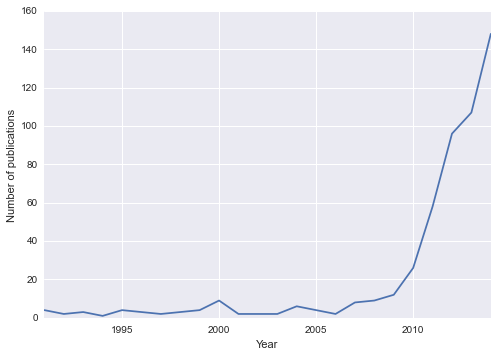
\includegraphics[scale=0.43]{./figures/growth}
	\caption{The number of publications related to NILM research. \protect\footnotemark}
	\label{fig:growth}
\end{figure}%
\footnotetext{Oliver Parson, \texttt{http://blog.oliverparson.co.uk/2015/03/overview-of-nilm-field.html}, 25 March 2015, (accessed 10 June 2015)}
Recent development within technology and the adoption of big data has influenced and researchers often refer to a recent explosion in the number of NILM publications. The figure \ref{fig:growth} shows the number of papers published per year, from which the upward trend since 2010 is clearly visible. This renewed interest is likely due to recent countrywide rollouts of smart meters. 

\begin{figure}[H]
	\label{fig:citations}
	\centering
	\begin{minipage}{.45\textwidth}
		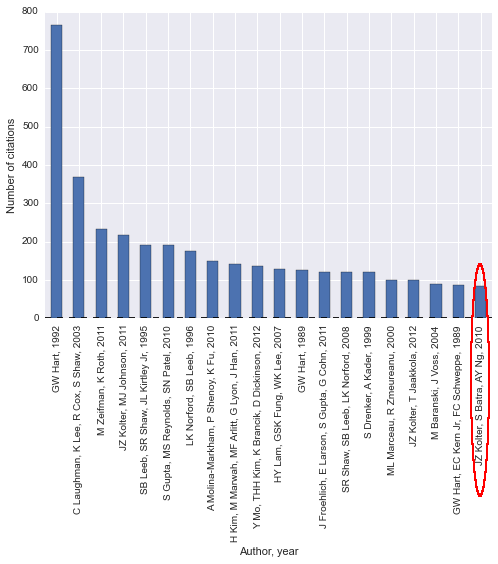
\includegraphics[scale=0.35]{./figures/citations_mod}
	\end{minipage}
	\begin{minipage}{.45\textwidth}
		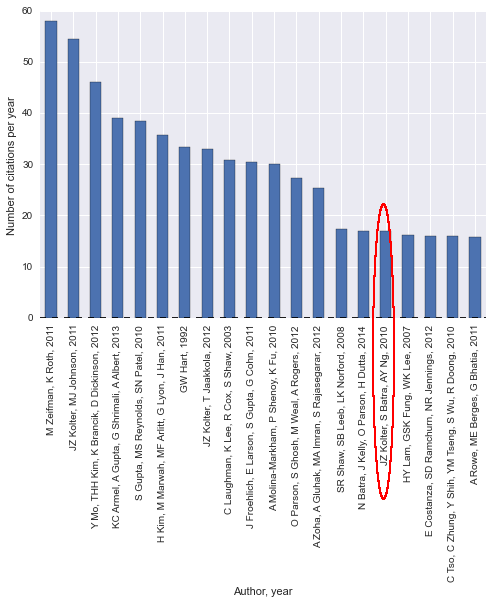
\includegraphics[scale=0.33]{./figures/citationsperyear_mod}
	\end{minipage}
	\caption{The figure shows citations of NILM related publications and highlights the paper by Kotler et. al \cite{DDSC}. The figure to the left shows number of citations overall, while the right figure show the number of citations for the year 2014. \protect\footnotemark}
\end{figure}

\footnotetext{Oliver Parson, \texttt{http://blog.oliverparson.co.uk/2015/03/overview-of-nilm-field.html}, 25 March 2015, (accessed 10 June 2015)}
Since older papers have had more time to accumulate citations, it's also interesting to look at citations per year to get a better idea of recent trends in the field, as shown by the graph on the right. Unlike before, there is no standout paper, with recent review papers and data set papers receiving the greatest citation velocity. One can see that the paper has not been the primary focus of research and is therefore interesting to look into. Besides these papers, a number of the remaining highly cited papers propose techniques based upon principled machine learning models. Most of the papers also focus on high-resolution data; in contrast, this thesis focuses on disaggregating electricity using low-resolution, hourly data of the type that is readily available via smart meters (but where most single-device “events” are not apparent); where we specifically look at temporal differences.

The method builds upon sparse coding methods and recent work in block-coordinate descent \cite{blondel,block2}. Specifically, we use a structured perceptron sparse coding algorithm presented in \cite{DDSC} using a coordinate descent approach to learn a model of each device’s power consumption over the specified time domains, week, two weeks and a month. While energy disaggregation can naturally be formulated as such a single-channel source separation problem, there is no previous application of these methods to the energy disaggregation task, until Kotler, Batra and Ng's algorithm \cite{DDSC}, presented in algorithm \ref{alg:ddsc}. Indeed, the most common application of such algorithm is audio signal separation, which typically has very high temporal resolution; thus, the low-resolution energy disaggregation task we consider here poses a new set of challenges for such methods, and existing approaches alone perform quite poorly. This thesis shows that the methods presented in \cite{DDSC} was cumbersome to implement and evaluate. The thesis also addressess the need for accurate energy consumption data, where the available dataset is far from being a good representation of the consumption inside a whole house. It also addresses that temporal differences have not affected the accuracy.

\subsection{Purpose}

The work described in this thesis was carried out at Greenely \protect\footnotemark. Greenely is a mobile application company based in Sweden, where a gamification model to educe a better energy consumption when providing consumers with their energy bills is being developed. Their solution is solely based on total energy consumption bills but would like to investigate a possible disaggregation for their costumers.

\footnotetext{Greenely, \texttt{http://greenely.com/about-us/}, 25 Feb 2015, (accessed 10 June 2015)}

The work has been to provide Greenely with steady insights of the energy disaggregation field as well as to implement Kotler et.al. models for a base model for energy disaggregation. The thesis aims to try to replicate their algorithm with using less data by using it on subsets of a larger dataset and therefore achieve reasonable disaggregation results. The performance results are presented and used for deciding whether or not to adopt the devised algorithm for their energy disaggregation.

\pagebreak[3]
\subsection{Thesis outline}
\label{sec:outline}
\begin{itemize}
	\item{Introduction}
	\begin{itemize}
		\item{\intOverview}
	\end{itemize}
	\item{Preliminaries}
	\begin{itemize}
		\item{}\preOverview
	\end{itemize}
	\item{Problem definition}
	\begin{itemize}
		\item{}\proOverview
	\end{itemize}
	\item{Fabrication}
	\begin{itemize} 
		\item{}\fabOverview
	\end{itemize}
	\item{Results}
	\begin{itemize}
		\item{}\resOverview
	\end{itemize}
	\item{Conclusions}
	\begin{itemize}
		\item{}\conOverview
	\end{itemize}
\end{itemize}